\documentclass[conference]{IEEEtran}
\IEEEoverridecommandlockouts
% The preceding line is only needed to identify funding in the first footnote. If that is unneeded, please comment it out.
\usepackage{amsmath,amssymb,amsfonts}
\usepackage{algorithmic}
\usepackage{graphicx}
\usepackage{textcomp}
\usepackage{listings}
\usepackage{hyperref}
\usepackage[T1]{fontenc}
\usepackage[utf8x]{inputenc}
\def\BibTeX{{\rm B\kern-.05em{\sc i\kern-.025em b}\kern-.08em
    T\kern-.1667em\lower.7ex\hbox{E}\kern-.125emX}}
\begin{document}

\lstset{basicstyle=\footnotesize\ttfamily,breaklines=true,literate={á}{{\'a}}1 {ê}{{\^e}}1 {é}{{\'e}}1 }

\title{Topic categorization in Portuguese news articles\\
\thanks{Fundação para a Ciência e Tecnologia} }


\author{\IEEEauthorblockN{André F. Santos}
\IEEEauthorblockA{\textit{CRACS \& INESC-Porto LA} \\ \textit{Faculty
of Sciences, University of Porto}\\ Porto, Portugal \\
afs@inesctec.pt} }

\maketitle

\begin{abstract} This document is a model and instructions for \LaTeX.
This and the IEEEtran.cls file define the components of your paper
[title, text, heads, etc.]. *CRITICAL: Do Not Use Symbols, Special
Characters, Footnotes, or Math in Paper Title or Abstract.
\end{abstract}

\begin{IEEEkeywords} topic categorization, machine learning, text
mining \end{IEEEkeywords}

\section{Introduction}
The last decades have witnessed a fast increase on the rate of publication
of digital text documents. Traditional document types, such as news
articles, scientific papers or books are now published online together
with new formats, such as blog posts or tweets, each having thousands
or millions of new documents published each day.

And it was not only the publication step which has moved to the
digital world; in fact, most often nowadays the whole document
lifecycle happens digitally, with virtual tools available for
preparing, writing, styling, publishing and sharing.

Having the entire workflow happening within the digital world presents
some opportunities when compared to the traditional process. In
particular, due to todays processing power, tasks related to the
manipulation of the information contained within these documents
(searching, compiling, annotating, sharing, \dots) can now be
performed automatically and targetting a large amount of articles.

In addition to the document content (for example, in a news article,
the \emph{title}, \emph{lead} and \emph{body}), its metadata is also
important: author(s), date of publication, source, topic, mentioned
entities and their relations, etc. Some of this metadata might be
filled in and stored along with the document (e.g. \emph{author} and
\emph{date of publication}); other is usually extracted from the
document content (e.g. mentioned entities).

Online news articles first appeared as reprints from traditional
newspapers; nowadays, however, they represent now the primary source
of news for some segments of the population, both in developed and
developing countries (whether consumed directly in the newspaper
website, or indirectly (e.g. through a social media application or a
feed catcher).

Unofficially know as \emph{the fourth branch of government}, the press
plays a vital role within our society, keeping us informed regarding
the current state of affairs (at a local and global scale) and acting
as a watchdog for the other three powers (legislative, executive and
judicial). The (lack of) freedom of press and access to the news in a
given country is even often considered an indicator of a lack of
democracy\cite{goode2009social}.

As such, improving the ways citizens can access the information (view
it, query it and search it) contained in news articles has the
potential to contribute for a more informed society and, ultimately, a
better society.

An example of a feature which improves information access is the
categorization of news articles by the topic (or topics) of its
content. The presence of such a categorization may influence the way
the information is stored, organized, displayed and queried.

The simplest way of achieving this categorization is to have the
author of the article to manually introduce it (e.g. the journalist
typing it on the news article authoring framework); however, this
solution presents some challenges:
\begin{itemize}
    \item it increases the amount of work the author has to do
    \item the author might not be sure which categories are available
    \item the author might not be sure which category is the best
        (e.g. \emph{Economics} vs  \emph{Finance})
    \item it does not scale -- e.g. if the goal is to categorize an
        existing (large) corpus
\end{itemize}

Thus, an automated way of categorizing news articles could solve some
of these problems and decrease the burden of this task.

The challenges of document classification have been well studied
within the machine learning research field of study. Given a corpus of
already classified documents, several algorithms might be applied to
train a classifier capable of determining the category of additional
articles.

In this article, we describe the preliminary results obtained in
developing a classifier to categorize news articles, and in developing
a similar classifier with restrictions added to the maximum size of
the lexicon used % TODO

\section{Methods}
%TODO
we first needed to choose and obtain a suitable dataset, and then
cleaning and preparing it to be used to train the classifiers.

\subsection{The dataset}
We gathered a dataset of news articles published in
\textit{Observador}\footnote{\url{http://observador.pt}}, one of the
main Portuguese newspapers, and which stands out from the others for
being fairly young (it was created in May 2014) and for existing
exclusively online. The initial dataset comprised 42.475 entries, from
which we used only a subset, for reasons later described.

We gathered all the categories used by Observador, and ordered them
from the most common to the least common. We selected the ones which
had more than 1.000 articles in our dataset, and reduced our original
dataset to include only articles from these categories.
Figure~\ref{fig:articles} presents an overview of the selected
categories and the number of articles available for each one.

\begin{figure}[htbp]
\centerline{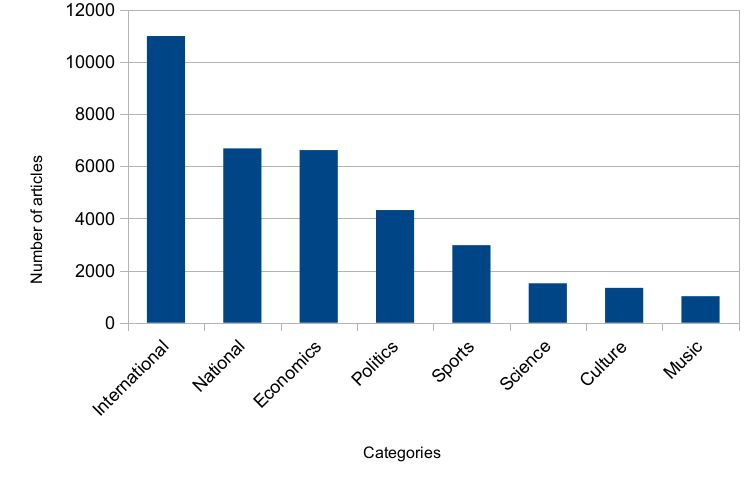
\includegraphics[width=.97\columnwidth]{imgs/articles}}
\caption{Total number of articles retrieved for each category}
\label{fig:articles}
\end{figure}

We them randomly selected, from each category, 700 articles to be used
to train the classifiers, and 200 to be used to evaluate their
performance.

For each article, we had available its contents (title, lead, body)
and several metadata fields (publication date, category, tags, etc). A
truncated JSON representation of an article can be found in
Listing~\ref{lst:article}.

\begin{lstlisting}[caption={Example of JSON representation of an article},label={lst:article}, extendedchars=true]
{
  Type: "sapo.obj.creativework.article",
  Source: {
      Name : "Observador"
  },
  Pretitle: "Benfica",
  Title: "Ruben Amorim com rotura total do ligamento cruzado",
  Author: {
      Name: "Observador"
  },
  Tags: [
      "benfica",
      "desporto",
      "futebol",
      "ruben amorim"
  ],
  PublishDate: ISODate("2014-08-25T18:33:00Z"),
  Lead: "Depois de Fejsa, mais uma baixa. O internacional português [...]",
  Body: "<p>O pior cenário confirmou-se. O Benfica informou esta segunda-feira [...]",
  URL: "http://observador.pt/2014/08/25/ruben-amorim-com-rotura-total-ligamento-cruzado/",
  CategoryPaths: [
      "Desporto"
  ],
  Domain: "observador.pt",
  Language: "pt_PT",
  ...
}
\end{lstlisting}

\subsection{Preprocessing the articles}

Originally, the dataset was obtained as large (more than 2.5 million
entries) MongoDB collection, containing articles from several
Portuguese and international newspapers. The process required to
transform this collection into data our classifiers could process
required: querying the database, exporting the news articles and
splitting them into a train and an evaluation datasets.

The database query selected articles from \texttt{Observador} where
the body had a length greater than 100 characters (to
discard some malformed articles which had an empty body or a body
composed of only a few words), and the categories included at least
one of the categories we previously selected.

For each article returned by the query, the pretitle, title, subtitle
and lead fields, if present, were simply copied to a plain text file,
separated by blank lines. The body field, however, was stored in the
database in HTML format. As such, the HTML tags had to be stripped,
and then it was also added to the plain text file.

The files were then stored in folders, separated by the category.
Furthermore, for each category, 700 articles were allocated to the
train set, and 200 to the evaluation set.

These preprocessing tasks were accomplished using Bash and Node.js
scripts.

\subsection{Classification algorithms}


\subsubsection{Decision tree}
\subsubsection{k-nearest neighbors}
\subsubsection{Naive Bayes}
\subsubsection{Neural network}
\subsubsection{Support vector machine}

\subsection{Most informative terms}
% for real-time topic suggestion (for an IDE for example)
% memory limit
% 100 terms? 1000 terms?

\section{Results}

\begin{table}[htbp]
    \caption{Categories confusion matrix (k-nearest neighbors)}
\begin{center}
\begin{tabular}{l|rrrrrrrr}
              & ciencia     & cultura     & desporto     & economia     & mundo       & musica       & pais        & politica \\\hline
ciencia       & \textbf{64} & 18          & 25           & 29           & 21          & 37           & 4           & 2 \\
cultura       & 4           & \textbf{37} & 16           & 9            & 19          & 107          & 3           & 5 \\
desporto      & 1           & 4           & \textbf{130} & 8            & 19          & 35           & 2           & 1 \\
economia      & 0           & 6           & 9            & \textbf{127} & 12          & 32           & 1           & 13 \\
mundo         & 9           & 8           & 25           & 31           & \textbf{82} & 32           & 1           & 12 \\
musica        & 0           & 6           & 1            & 1            & 0           & \textbf{180} & 0           & 1 \\
pais          & 8           & 15          & 24           & 42           & 17          & 64           & \textbf{14} & 16 \\
politica      & 1           & 8           & 7            & 36           & 19          & 24           & 3           & \textbf{102} \\

\end{tabular}
\label{tab1}
\end{center}
\end{table}
% >\\  error.rate.knn
% [1] 0.5368156
\subsection{Evaluation}
\subsection{Limited lexicon}

\section{Discussion}
% nested categories
% or not mutex categories


\section*{Acknowledgment}

André Santos has a scholarship from Fundação para a
Computação Científica Nacional.

\bibliography{article}
\bibliographystyle{splncs03}

\end{document}
